% vim: set tw=0:
\documentclass{beamer}
\usepackage{graphicx}
\usepackage{hyperref}
\hypersetup{pdfborder={0 0 0 0}}

% Reasonable themes:
% Antibes Bergen Berkeley Berlin Frankfurt Goettingen Ilmenau Luebeck Malmoe
% Montpellier PaloAlto Rochester Singapore Szeged Warsaw bars boxes
% compatibility default lined plain shadow sidebar split tree
% And these ones include the author's name on every slide:
% Berkeley

% Declare themes.
\mode<presentation>
\usetheme{UWHEP}

% Personal macros.
\newcommand{\email}[1]{{\texttt #1}}
\newcommand{\newframe}[1]{\section{#1}
    \frametitle{\sc{#1}}}
\newcommand{\subframe}[1]{\subsection{#1}
    \frametitle{\sc{#1}}}
\newcommand{\supers}[1]{\ensuremath{^\textrm{#1}}}
\newcommand{\subs}[1]{\ensuremath{_\textrm{#1}}}
\newcommand{\ca}{\ensuremath{\sim}}
\renewcommand{\email}[1]{\href{mailto:#1}{\nolinkurl{#1}}}

% Author information.
\title{Storage at UW-Madison CMS Tier-2}
\author[Maier]{
    Will Maier \\ 
    {\tt wcmaier@hep.wisc.edu}}
\institute[Wisconsin]{University of Wisconsin - High Energy Physics}
\date[2010.09.22]{OSG Storage Forum, U. Chicago}
\logo{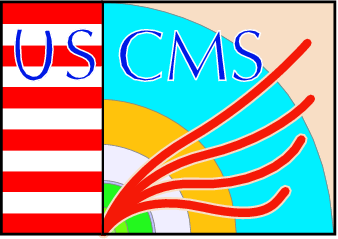
\includegraphics[height=0.6cm]{../../../Graphics/USCMS_logo.png}\hspace{.1cm}
\includegraphics[height=0.75cm]{../../../Graphics/UW_logo.png}}

\begin{document}

% http://indico.fnal.gov/conferenceTimeTable.py?confId=3377
% 15 min
% hardware/layout
% software
% monitoring/management
% evaluation
% plans

\begin{frame}
    \titlepage
\end{frame}

\section{Overview}
\begin{frame}
    \tableofcontents
\end{frame}

\section{Hardware}
\subsection{Summary}
\subsection{Core}
\begin{frame}
\begin{itemize}
	\item Four core dCache machines: PNFS, admin/misc, doors, hotspare
	\item 1 Gbps connections, SATA disks, 2x2 2.0 GHz Opterons, 16 GB RAM
	\item PNFS: RAID10 (10kRPM disks), 2x4 3.0 GHz Xeons
	\begin{itemize}
		\item Current configuration \ca{}12 months old
		\item Nearly saturated (again)\ldots{}need more IO
	\end{itemize}
	\item admin, doors, hotspare: commodity, nothing special
	\begin{itemize}
		\item No observed scaling issues with shared SRM/dcap door
		\item \ca{}32 GridFTP doors live on data nodes (easy to add more)
	\end{itemize}
	% plot requests/time? files?
\end{itemize}
\end{frame}

\subsection{Cluster}
\begin{frame}
\begin{itemize}
	\item \ca{}50\% dedicated, \ca{}50\% shared with compute resources
	\item Dedicated nodes: mix of RAID6, RAID0 with 1 - 2 TB SATA disks
	\item Shared nodes: no RAID, .5 - 2 TB SATA disks (4 - 16 slots, 2 - 48 GB RAM)
	\item XXX pools on XXX nodes
	\item XXX Gbps network managed by campus
	% plot: TB/time
\end{itemize}
\end{frame}

\section{Software}
\subsection{Platform}
\begin{frame}
\begin{itemize}
	\item Scientific Linux 5.3/kickstart
	\item dCache v XXX
	\item SRM v XXX, gsiftp v XXX
	\item xrootd redirector thingy XXX
	% plot XXX
\end{itemize}
\end{frame}

\section{Management}
\subsection{Management} % cli, dcache_tools, dcache info provider
\begin{frame}
	\item Install nodes with kickstart, manage live configuration with Cfengine (v2)
	\item Management scripts written with dcache-tools~\footnote{\url{http://code.hep.wisc.edu/dcache-tools}}, based on CLI~\footnote{\url{http://packages.python.org/pyCLI}}
	\begin{itemize}
		\item {\tt dcache_absent}: List absent and offline pools
		\item {\tt dcache_billingrep}: Watch billing log and initiate replications of new files
		\item {\tt dcache_clean}: Remove invalid/unlinked files directly from pools
		\item {\tt dcache_df}: {\tt df(1)}-like overview of cluster storage
		\item etc\ldots{}
	\end{itemize}
	\item Less web scraping, more dCache info provider
	\begin{itemize}
		\item Previously, most monitors/checks polled dCache web pages and scraped HTML
		\item Info provider allows simple XML parsing (and exposes lots of detail)
		\item Can request subsets of data (ie for {\tt dcache_df})
		% XXX: output?
	\end{itemize}
\end{frame}

\subsection{Alerts and Trends} % nagios
\begin{frame}
\begin{itemize}
	\item Nagios checks for all servers in both the core and cluster
	\item Some Nagios protocol checks (GridFTP, SSH admin interface)
	\item Functional tests via cron jobs (SRM/dcap/GridFTP read/write)
	\item External monitoring (CMS SAM/JobRobot/Dashboard/SiteView/PhEDEx, OSG RSV, MyOSG, Gratia, \ldots{})
	\item Aggregate local monitoring in tsar
\end{itemize}
\end{frame}

\subsection{Trends} % tsar
\begin{frame}
\begin{itemize}
	\item 
\end{itemize}
\end{frame}

\section{Evaluation}
\subsection{What Works}
\subsection{What Doesn't}
% dcache hotspots

\section{Plans}
\begin{frame}
\begin{itemize}
	\item Centralize dCache logging
	\item Scale tsar
	\item Explore HDFS w/ xrootd frontend (to support jobs on local opportunistic resources)
	\item PNFS $\rightarrow$ Chimera? dCache $\rightarrow$ HDFS?
\end{itemize}
\end{frame}

\end{document}
